\lhead{\textbf{Basic Algorithms, Fall 2024 \\ CSCI-UA.0310-001}}
\chead{\Large{\textbf{Homework 7}}}
\def\lc{\left\lceil}   
\def\rc{\right\rceil}
\rhead{\textbf{Instructor: Rotem Oshman \\Name: Ishan Pranav}}
\runningheadrule
\firstpageheadrule
\cfoot{}
\subsection*{References}
Collaborated with Crystal Huang.
\stepcounter{subsection}
\subsection{Huffman codes}
\begin{enumerate}
\item 
Consider a file that uses the following list of symbols with the corresponding frequencies:
\begin{center}
\begin{tabular}{|c|c|c|c|c|c|c|c|}
\hline
     Letter & A & B & C & D & E & F & G\\
     \hline 
     Frequency & 0.06 & 0.09 & 0.10 & 0.12 & 0.15 & 0.16 & 0.32\\
     \hline
\end{tabular}
\end{center}

\noindent Find an optimal prefix code based on Huffman's algorithm (using the symbols $0$ and $1$ only). Work out the code by drawing the tree and then describing the mapping from symbols to bit strings.
\begin{figure}[h]
\centering
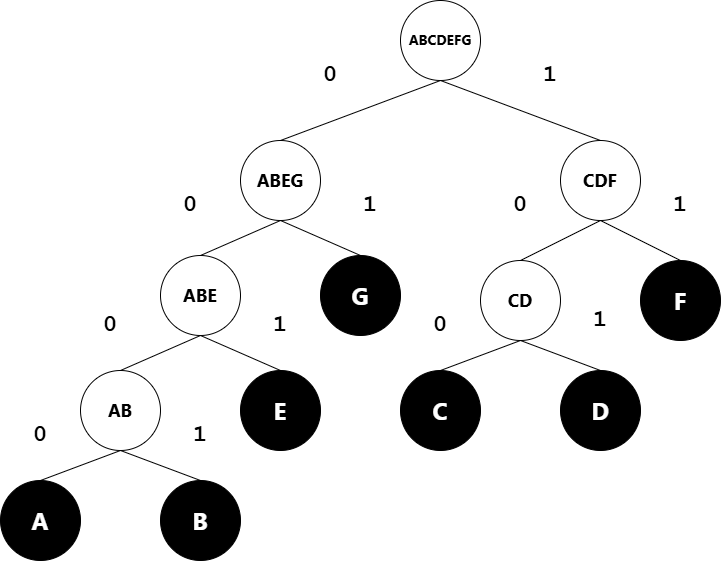
\includegraphics[width=9.5cm]{../images/hw7-1-1.png}
\caption{A Huffman tree for the given list of symbols and their frequencies, constructed using Huffman's algorithm.}
\label{fig:hw7_1_1}
\end{figure}

\begin{solution}
We can step through the recursive levels of Huffman's algorithm to construct a Huffman tree and obtain an optimal prefix code.

\textit{First. }The two lowest-frequency symbols are A and B with $f_{\rm A}=0.06$ and $f_{\rm B}=0.09$, respectively. We replace them with the pseudo-symbol AB such that $f_{\rm AB}=0.06+0.09=0.15$.

\textit{Second. }The two lowest-frequency symbols are C and D with $f_{\rm C}=0.10$ and $f_{\rm D}=0.12$, respectively. We replace them with the pseudo-symbol CD such that $f_{\rm CD}=0.10+0.12=0.22$.

\textit{Third. }The two lowest-frequency symbols are AB and E with $f_{\rm AB}=f_{\rm E}=0.15$. We replace them with the pseudo-symbol ABE such that $f_{\rm ABE}=0.15+0.15=0.30$.

\textit{Fourth. }The two lowest-frequency symbols are F and CD with $f_{\rm F}=0.16$ and $f_{\rm CD}=0.22$. We replace them with the pseudo-symbol CDF such that $f_{\rm CDF}=0.16+0.22=0.38$.

\textit{Fifth. }The two lowest-frequency symbols are ABE and G with $f_{\rm ABE}=0.30$ and $f_{\rm G}=0.32$. We replace them with the pseudo-symbol ABEG such that $f_{\rm ABEG}=0.30+0.32=0.62$.

\textit{Sixth. }The two remaining symbols are ABEG and CDF. We construct parent vertex ABCDEFG and take ABEG and CDF to be children of ABCDEFG.

Then, we reconstruct the tree by unwinding the recursion and re-attaching the terminal symbols, taking the psuedo-symbols to be their parent vertices. Finally, we can arbitrarily assign all left edges to represent a $0$ bit and all right edges to represent a $1$ bit. See Figure~\ref{fig:hw7_1_1}.

We can now construct the optimal prefix code for each symbol by traversing the tree from root to leaf and taking note of the edges followed:

\begin{center}
\begin{tabular}{c|c}
Letter&Encoding\\
A&0000\\
B&0001\\
C&100\\
D&111\\
E&001\\
F&11\\
G&01\\
\end{tabular}
\end{center}
This completes our encoding.
\end{solution}
\newpage
\item In general, are Huffman codes unique? That is, for a given set of letters and corresponding frequencies is there a unique Huffman encoding? Note that different letters may have the same frequency in the general case. If yes, justify. Otherwise provide a counterexample.
\begin{solution}
No, in general, Huffman codes are not unique.

First, bits are assigned to edges arbitrarily. For a given parent vertex, it is possible to let its left edge represent the $0$ bit and the right edge represent the $1$ bit, or to let the right represent $1$ and the left represent $0$. The only constraint on the assignment of bits is that one side must represent $0$ and the other must represent $1$. 

Furthermore, we can show that Huffman codes are not unique even with a consistent constraint on the assignment of the bits. 

Without loss of generality, assume that for every parent vertex, we always let its left child represent the $0$ bit and the right child represent the $1$ bit.

Consider four A, B, and C, with frequencies $f_{\rm A}=f_{\rm B}=f_{\rm C}=0.\overline{3}$. We want to construct an optimal prefix code using Huffman's algorithm. On the first recursive level, we may choose any of A and B, B and C, or C and A to be the two lowest-frequency symbols. Consider two of these cases:
\begin{itemize}
\item Suppose we take A and B to be the two lowest-frequency symbols. Then we replace them with parent AB with frequency $f_{\rm AB}=0.\overline{6}$, with A as the left child and B as the right. Now AB and C are joined to a parent to construct the tree, with AB as the left child and C as the right.

In our optimal Huffman code, we represent A with $01$, B with $00$, and C with $1$.

\item Suppose instead we take B and C to be the two lowest-frequency symbols. Then we replace them with parent BC with frequency $f_{\rm BC}=0.\overline{6}$, with C as the left child and b as the right. Now A and BC are joined to a parent to construct the tree, with A as the left child and C as the right.

In our optimal Huffman code, we represent A with $0$, B with $10$ and C with $11$.
\end{itemize}
We have shown that with the same list of symbols and frequencies, Huffman's algorithm may produce entirely different optimal prefix codes. Thus, Huffman codes are not unique.
\end{solution}
\end{enumerate}
\newpage
\subsection{Minimizing number of colors}
Let $X$ be a set of $n$ intervals $[s_i, f_i)$ on the real line. A {\em proper coloring} of $X$ assigns a color to each interval so that overlapping intervals are always assigned different colors.  In this problem, we want to find a proper coloring of $X$ using a minimum possible number of colors. Let us call this (unknown) number $c^*$.
\begin{enumerate}
\item Given a problem instance $\{[s_i,f_i)\}$ and any point on the real line $t$, let $n_t$ denote the number of sets that contain $t$. Also, let $c = \max_t n_t$ (easy to see the maximum is well defined). Argue that $c^*\ge c$.
\begin{solution}
\textbf{Proposition I. }
\textit{Claim. }Let $X$ be a set of $n$ real intervals $[s_i,f_i)$ for $1\leq i\leq n$. For all $t\in\mathbb{R}$, let $n_t$ denote the number of intervals $x\in X$ where $t\in x$. Let $c=\underset{t\in\mathbb{R}}{\max}(n_t)$. Let $c^*$ be the minimum number of colors required to produce a proper of coloring of $X$. Then $c^*\geq c$.

\textit{Proof. }Since there exists $c=\underset{t\in\mathbb{R}}{\max}(n_t)$, there exists $t^*\in\mathbb{R}$ where $c=n_{t^*}$.

By definition, there are $n_{t^*}$ intervals $x\in X$ where $t^*\in x$. So, $n_{t^*}$ intervals overlap at the point $t^*$. In a proper coloring of $X$, each of these $n_{t^*}$ overlapping intervals is assigned a unique color. This implies that there are at least $n_{t^*}$ colors in a proper coloring of $X$. Since $c^*$ is the minimum number of colors required to produce a proper coloring of $X$, we know $c^*\geq n_{t^*}$.

Of course, $c=n_{t^*}$. Ergo $c^*\geq c.~\square$
\end{solution}
\newpage
\item Consider the following greedy algorithm for solving this problem.
\vspace*{-1ex}
\begin{code}
\> Sort the intervals according to $s_i$. \\
\> Initialize the current number $z$ of defined colors to $0$. \\
\> \For $i = 1$ to $n$, perform the following greedy step. \\
\> \> \If next interval $a_i = [s_i, f_i)$ cannot be legally colored
with any color $1\le j\le z$\\
\> \> \Then increment $z$ by $1$ and assign $a_i$ the new color $z$.\\
\> \> \Else color $a_i$ with the smallest ``legal'' color
$j\in \{1, \ldots, z\}$
\end{code}
Argue that the greedy algorithm above computes a valid coloring, and yet {\em never uses more than $c$ colors}, where $c$ is the quantity from part (a).%\hint{Assume the intervals to be sorted according to $s_i$ and prove the statement using induction.}
\begin{solution}

\textbf{Algorithm I. }{\sc GreedyAlgorithm}($X$), where $X$ is a set of $n$ real intervals $[s_i,f_i)$ for $1\leq i\leq n$.

For all $t\in\mathbb{R}$, let $n_t$ denote the number of intervals $x\in X$ where $t\in x$. Let $c=\underset{t\in\mathbb{R}}{\max}(n_t)$. 

Assume without loss of generality that the intervals are sorted in ascending order with respect to their starting value. That is, for all $1\leq p<q\leq n$, we have $[s_p,f_p)\in X$ and $[s_q,f_q)\in X$ such that $s_p\leq s_q$.

Let $1\leq j\leq(n+1)$ where $j=1$ denotes the iteration before the loop begins, $j=i$ denotes the iteration before considering interval $[s_i,f_i)\in X$ for $i\leq n$, and $j=n+1$ denotes the step immediately after the loop terminates.

Let $z_j$ denote the number of unique colors used at the beginning of iteration $j$.

\textbf{Invariant I. }\textit{Claim. }For every step of the loop $1\leq j\leq(n+1)$, we claim that
\begin{itemize}
\item there exist no $p$, $q$, and $t$ where $1\leq (p\neq q)<j\leq n$ such that $t\in[s_p,f_p)$ and $t\in[s_q,f_q)$, but $[s_p,f_p)$ and $[s_q,f_q)$ have the same color; and,
\item$z_j\leq\underset{t\in\mathbb{R}}{\max}({n_j}_t)$ where ${n_j}_t$ denotes the number of intervals $[s_i,f_i)\in X$ where $i<j$.
\end{itemize}
\textit{Proof. }We can prove this invariant by induction on $j$.

\textit{Basis. }Consider $j=1$. Note that we are considering the case before the first iteration of the loop.

Since $j=1$, there are no intervals $[s_i,f_i)\in X$ where $i<1$, as no intervals have yet been considered.

It follows that ${n_1}_t=0$ for all $t\in\mathbb{R}$. From Algorithm I, before the loop begins, $z_1=0$. So $z_1\leq\underset{t\in\mathbb{R}}{\max}({n_1}_t)$.

Thus the loop invariant holds at initialization.

\textit{Hypothesis. }Consider $j=k$ where $1\leq k\leq n$. Assume that at the beginning of iteration $k$,
\begin{itemize}
\item there exist no $1\leq (p\neq q)<k\leq n$ where $[s_p,f_p)\in X$ and $[s_q,f_q)\in X$ are overlapping intervals with the same color; and,
\item$z_k\leq\underset{t\in\mathbb{R}}{\max}({n_k}_t).$
\end{itemize}
\textit{Inductive step. }Consider $j=k+1$. Note that this is the iteration immediately after considering interval $k$ and before considering interval $k+1$. There are two cases.
\begin{itemize}
\item Suppose $[s_k,f_k)$ cannot be legally colored with any color $1\leq y\leq z$.
\item Suppose instead $[s_k,f_k)$ can be legally colored with some color $1\leq y\leq z$.
\end{itemize}
\textbf{Proposition II. }
\textit{Claim. }Algorithm I produces a proper coloring using no more than $c$ colors.

\textit{Proof. }Algorithm I terminates when its loop terminates; that is, it terminates when $i=n$ on iteration $j=n+1$.

From Invariant I, at termination there is no pair of distinct overlapping intervals with the same color. Therefore, Algorithm I computes a proper coloring of $X$.

At termination, the number of colors used is $z=z_{n+1}$. From Invariant I, $z_{n+1}\leq c$. Therefore, Algorithm I uses $z\leq c$ unique colors.

Ergo, {\sc GreedyAlgorithm}($X$) produces a proper coloring of $X$ using $z\leq c$ unique colors.
\end{solution}
\item What is the running time of this algorithm as a function of $n$ and $c^*$?
\begin{solution}
\textbf{Proposition III. }\textit{Claim. } Let $c^*$ be the minimum number of colors required to produce a proper of coloring of $X$. Then {\sc GreedyAlgorithm}($X$) has running time $O(n\log n+nc^*)$.

In the worst case, all intervals overlap, so $c^*=n$ and the running time is $O(n^2)$.

\textit{Proof. }First, {\sc GreedyAlgorithm}($X$) sorts the $n$ intervals in $X$. This is an $O(n\log n)$ process.

Then, for each of the $n$ intervals in $X$, the algorithm performs the main loop. In the worst case, the loop body considers all $z$ previously-defined colors from $1$ to $z$ before determining that no such color is legal for the current interval. Of course, $z=c$ in the worst case. This is an $O(c)$ process. The loop body always branches, sometimes increments $z$, and always assigns $z$ to the current interval: these execute in $O(1)$ time. So the loop body is an $O(c)+O(1)=O(c)$ process. Thus, the worst-case running time of the loop is $O(nc)$.

Therefore, the running time of Algorithm I is $O(n\log n)+O(nc)=O(n\log n+nc)$.

From Proposition I, we have $c^*\geq c$. Ergo Algorithm I has running time $O(n\log n+nc^*).~\square$
\end{solution}
\end{enumerate}